\begin{figure}[h!]
\textbf{Tema d'Esame di Gennaio 2015}\\ \\
Una molla con costante elastica $k=130N/cm$ viene compressa di $10 cm$ prima di lanciare una pallina di massa $40g$ verso un piano inclinato. Qual'è l'altezza massima dal suolo che raggiunge la pallina?
\\
	\begin{center}
		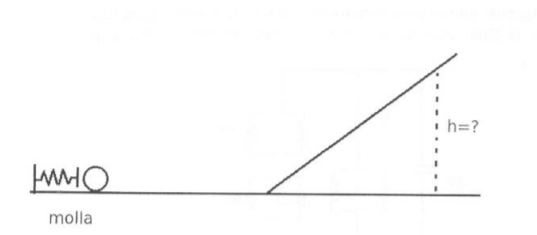
\includegraphics[scale=0.5]{ES2/GEN022015.jpg}
	\end{center}
\end{figure}

\begin{figure}[h!]
\textbf{Tema d'Esame di Febbraio 2015}\\ \\
Una molla ideale può essere compressa di $1.0 m$ da una forza di $100 N$. La stessa molla è
posta alla fine di un piano inclinato liscio (senza attrito) che forma un angolo di $30^{\circ}$ con l'orizzontale. Una massa $M$ di $10 kg$ viene lasciata cadere da ferma dal vertice del piano inclinato e si arresta momentaneamente dopo aver compresso la molla di $2.0 m$. Qual'è la velocità della massa un attimo prima di toccare la molla? 
\\
	\begin{center}
		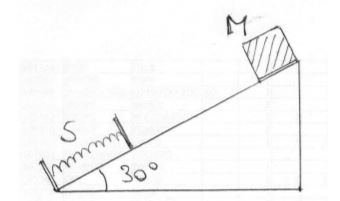
\includegraphics[scale=0.6]{ES2/FEB022015.jpg}
	\end{center}
	
\end{figure}

\begin{figure}[h!]
\textbf{Tema d'Esame di Giugno 2015}\\ \\
Una molla con costante elastica $75=75N/cm$ viene compressa di $20 cm$ prima di lanciare una pallina ($m=80g$) verso un piano inclinato. Qual'è l'altezza massima dal suolo che raggiunge la pallina? 
\\
	\begin{center}
		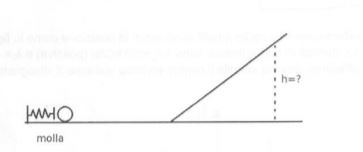
\includegraphics[scale=0.9]{ES2/GIU022015.jpg}
	\end{center}
\end{figure}

\begin{figure}[h!]
\textbf{Tema d'Esame di Luglio 2015}\\ \\
Una pallina ($m=100g$) viene lanciata con velocità di $2km/h$ da un punto su un piano orizzontale alla sommità di un piano inclinato alto $120cm$.
Quando la pallina scende dal piano incontra una molla con costante elastica $k=1N/cm$. Di quanto si comprime la molla per fermare la pallina? 
\\
	\begin{center}
		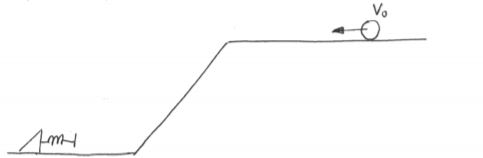
\includegraphics[scale=0.7]{ES2/LUG022015.jpg}
	\end{center}
	
\end{figure}

